\documentclass{article}
\usepackage{graphicx}
\usepackage{float}
\usepackage{gensymb}
\parskip=12pt

\begin{document}

\title{Laboratory 5: Geometric Optics}
\date{December 3, 2014}
\author{Calvin Chan\\304144970\\Physics 4BL Lab 8\\Partners: Caleb Choi, Stanley
Chan}

\maketitle

\section{Introduction}

This lab aims to demonstrate various optical theories. By sending a ray through
a trapezoidal prism, we can observe the incident and refracted angles of the
ray, thus calculating the theoretical value of the index of refraction. We can
then verify Snell's law by physically finding the critical angle of the prism to
see how the experimental and theoretical values of the index of refraction
compare.

Following that, We measure the focal lengths of three lenses biconcave,
plano-convex, and biconvex. We can shine rays through the lenses and observe
where the rays converge, whether it's before or after the lens. By isolating and
removing certain rays, we can observe the effects of spherical aberration.
Additionally, we can observe the effects of magnification through the biconcave
and biconvex lenses by measuring the distance between the rays before and after
the rays are refracted. Finally, we can shine the rays through thin lenses and
observe where the rays converge (focal length). This final experiment can be
used to verify the equation of a combination of lenses and the image-object
equation.

\section{Experimental Results}

\subsection{Snell's Law and Total Internal Reflection}

A monochromatic ray of light was shot into a trapezoidal prism as shown in
figure \ref{trapezoidal_prism}. We measured the incident and transmitted angles
of the ray (both measured against the normal of the front interface)
to be $33\degree$ (0.576 rad) and $19\degree$ (0.332 rad), respectively.

\begin{figure}[H]
    \centering
    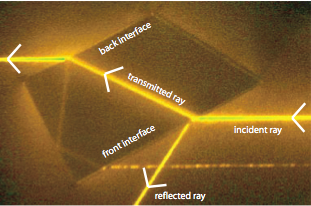
\includegraphics[width=0.7\textwidth]{charts/trapezoidal_prism}
    \caption{The trapezoidal prism}
    \label{trapezoidal_prism}
\end{figure}

We measured then measured the angles of the ray as it exited the prism through
the back interface. Inside the prism, it approached the back interface at an
angle of $18 \degree$ (0.314 rad) to the normal, and exited with an angle of $32
\degree$ (0.559 rad) to the normal.

We then used a similar method to find the critical angle for the prism – the
angle of incidence at which there is no refraction, but just total internal
reflection inside the prism. We measured the incident angle of ray to the front
interface to be $27 \degree$ (0.471 rad) and the angle of the transmitted ray
inside the prism to be $16 \degree$ (0.279 rad). The critical angle inside the
prism was measured to be $44 \degree$ (0.768 rad), the incident angle as the ray
approached the edge from within the prism itself.

\subsection{Thick Lenses}

\begin{figure}[H]
    \centering
    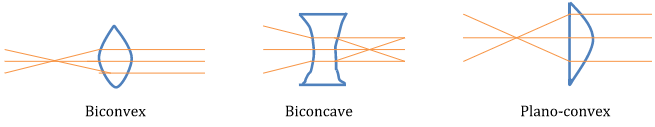
\includegraphics[width=\textwidth]{charts/thick_lenses}
    \caption{Using the ray box, light rays were shined into various thick lenses
    from the right to observe their focal lengths}
    \label{thick_lenses}
\end{figure}

For this section of the lab, we measured the focal lengths of various thick
lenses: biconcave, biconvex, and plano-convex (ref. figure \ref{thick_lenses}).
For the biconcave lens, we used the ray box to shine three rays at the lens,
tracing the diverging rays back to one point before the lens. We then measured
the distance between the lens and the point to be $30.5mm$, the focal length of
the biconcave lens. Similarly, we shined three rays at the biconvex lens and the
rays converged on the other side of the lens, a distance of  $58mm$ away from
the lens. We performed the same process on plano-convex lens, and recorded the
convergence of the rays at a distance of $94mm$ away from the lens. The
following chart shows the focal lengths of all the thick lenses. 

\begin{figure}[H]
    \centering
    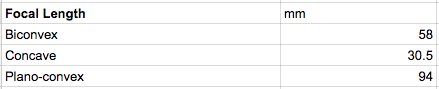
\includegraphics[width=0.7\textwidth]{charts/thick_lenses_focal_length}
    \caption{Focal lengths for various thick lenses}
    \label{thick_lenses_focal_length}
\end{figure}

\begin{figure}[H]
    \centering
    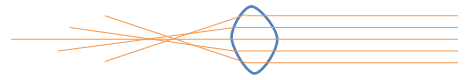
\includegraphics[width=0.7\textwidth]{charts/spherical_aberration}
    \caption{Spherical aberration exhibited by the biconvex lens}
    \label{spherical_aberration}
\end{figure}

Next, we used the ray box to shine 5 parallel rays of light into a biconvex
lens (figure \ref{spherical_aberration}). We could observe the effects of
spherical aberration through the rays near the edge of the lens, as they
effectively had a different focal point than the three inner rays. We measured
the positions of both focal points and determined the distance between them, as
shown in the following chart.

\begin{figure}[H]
    \centering
    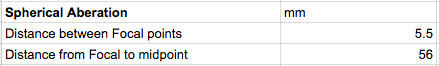
\includegraphics[width=0.7\textwidth]{charts/thick_lenses_spherical_aberration}
    \caption{Distances between focal points due to spherical aberration}
    \label{thick_lenses_spherical_aberration}
\end{figure}

\begin{figure}[H]
    \centering
    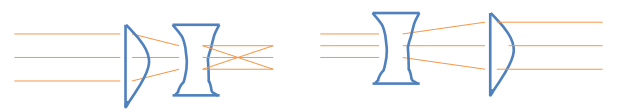
\includegraphics[width=0.7\textwidth]{charts/magnification}
    \caption{Combining two lenses to experiment with magnification and
    demagnification}
    \label{magnification}
\end{figure}

Finally, we used both, the biconvex lens and the biconcave lens together to observe
magnification properties of the lenses (figure \ref{magnification}). Using the
ray box, we shined three rays of light into the biconvex lens followed by a
biconcave lens to demonstrate demagnification. We then switched the order of the
lenses (biconcave followed by biconvex) and experimented with various distances
between the lens and ray box to find the maximum magnification. We measured the
distances between the rays before and after the magnification and
demagnification, as shown in the following chart.

\begin{figure}[H]
    \centering
    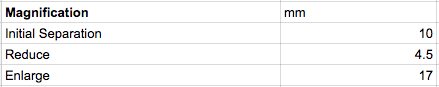
\includegraphics[width=0.7\textwidth]{charts/thick_lenses_magnification}
    \caption{Magnification through biconvex and biconcave lenses}
    \label{thick_lenses_magnification}
\end{figure}

\subsection{Thin Lenses}

For this part of the experiment, a beam splitter was used to shine two parallel
laser light beams of monochromatic light into various thin lenses, which would
result in the refraction and eventual convergence of those beams at some distance
from the lens. We measured the distance at which the beams started to converge
and started to diverge, obtaining the focal length of each lens by taking the
average of such measurements. The following charts shows our results:

\begin{figure}[H]
    \centering
    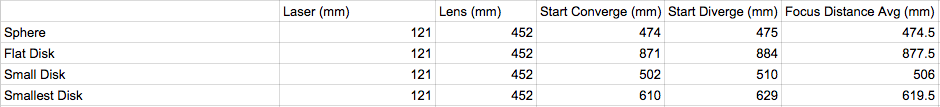
\includegraphics[width=\textwidth]{charts/thin_lenses}
    \caption{Finding the focal length of various thin lenses}
    \label{thin_lenses}
\end{figure}

Each final focus distance measurement had an uncertainty of $0.4mm$.

\begin{figure}[H]
    \centering
    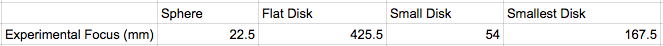
\includegraphics[width=\textwidth]{charts/thin_lenses_results}
    \caption{The focal lengths of various thin lenses}
    \label{thin_lenses_results}
\end{figure}

Each experimental focal length had an uncertainty of $0.8mm$.

Furthermore, we also combined the flat and the small disks and observed that the
combination had an experimental focal length of $50mm \pm 0.5mm$ (the disks were
8mm apart).

\subsection{Image Formation with Lenses}

For the final portion of the lab, we shined a LED through a $1mm$ grating.
The LED and the grating were placed behind a lens and a screen was placed on the
other side of the lens. To create the sharpest image possible, we experimented
with various distances between the LED grating and the lens, and between the
lens and the screen. Using the same method from the previous part of the lab
(averaging the focal distances), we obtained the following data:

\begin{figure}[H]
    \centering
    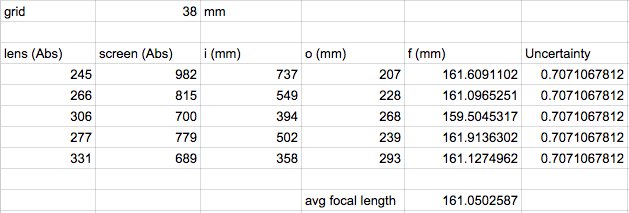
\includegraphics[width=\textwidth]{charts/image_formation}
    \caption{Measuring the focal lengths at different distances}
    \label{image_formation}
\end{figure}

\section{Analysis}

\subsection{Snell's Law and Total Internal Reflection}

Using the angles we recorded (incident and transimitted) from the first part of
the lab, we can use Snell's Law (eq. \ref{snells_law}) to calculate the index of
refraction of the trapezoidal prism.

\begin{equation}
    \label{snells_law}
    n_{i}sin\theta_{i} = n_{t}sin\theta_{t}
\end{equation}

Since our incident medium is air, then we know that $n_{i}=1$, thus we can
calculate for $n_{t}$.

\begin{equation}
    \label{snells_law_1}
    (1)sin(33\degree) = n_{t}sin(19\degree)
\end{equation}
\begin{equation}
    \label{snells_law_2}
    n_{t} = 1.67
\end{equation}

With error propogation, we can report the following:

\begin{equation}
    \label{snells_law_3}
    n_{t} = 1.67 \pm 0.2235
\end{equation}

Using the calculated value for the index of refraction of the trapezoidal prism,
we can compute the theoretical value for the critical angle that would result in
total internal reflection.

\begin{equation}
    \label{total_internal_reflection_1}
    sin\theta_{c} = \frac{n_{t}}{n_{i}}
\end{equation}
\begin{equation}
    \label{total_internal_reflection_2}
    sin\theta_{c} = \frac{1}{1.67}
\end{equation}
\begin{equation}
    \label{total_internal_reflection_3}
    sin\theta_{c} = 36.8\degree \pm 0.43\degree
\end{equation}

We can see that our computed theoretical value for the critical angle is a few
degrees less than our experimental value ($44\degree$), even with the
uncertainty factored in. This error could have been caused by the limited
precision of our measurement, since we could not accurately determine one
precise value of the beam reflection. The manual measurements using a
protractor could have easily yielded large errors due to a false zero value and
the reflected laser beam itself had a large width with a variety of values we
could have used for the critical angle.

\subsection{Thick Lenses}

Using the distance measurements between light rays before and after
magnification, we can determine the magnification factor of the lenses:

\begin{equation}
    \label{magnification_factor_1}
    M = \frac{final separation}{initial separation}
\end{equation}
\begin{equation}
    \label{magnification_factor_2}
    M = \frac{17}{10}
\end{equation}
\begin{equation}
    \label{magnification_factor_3}
    M = 1.7 \pm 0.3
\end{equation}

\subsection{Thin Lenses}

When two thin lenses are placed next to each other in a sequence they form a
combined lens with focal length $f_{total}$ as defined by the following
equation:

\begin{equation}
    \label{lens_combo_1}
    \frac{1}{f_{total}} = \frac{1}{f_{1}}+\frac{1}{f_{2}}-\frac{e}{f_{1}f_{2}}
\end{equation}

In eq. \ref{lens_combo_1}, $e$ represents the distance between the two lenses.
As such, we can compute the theoretical value of the flat and small disk
combination by using the focal lengths of each individual disk respectively.

\begin{equation}
    \label{lens_combo_1}
    \frac{1}{f_{total}} = \frac{1}{425.5}+\frac{1}{54}-\frac{8}{(425.5)(54)}
\end{equation}
\begin{equation}
    \label{lens_combo_1}
    f_{total} = 49.01mm \pm 0.67mm
\end{equation}

As such, we can see that our theoretial value for the focal length of the flat
and small disk combo falls under the value we obtained experimentally taking
into account uncertainty and error propogation ($49mm
\pm 1mm$).

\subsection{Image Formation with Lenses}

The position of an image formed by an object illuminated on a thin filmis given
by the following equation:

\begin{equation}
    \label{image_formation_eq}
    \frac{1}{f} = \frac{1}{o}+\frac{1}{i}
\end{equation}

As shown in chart \ref{image_formation}, we applied equation
\ref{image_formation_eq} to our measured values of the object and image
distances to determine the focal length for different distances. We then
averaged all of the focal lengths obtained from different distances to determine
the average focal length for the lens itself ($161.05mm \pm 0.707mm$). The
theoretical value for the focal length is $167.5mm$ (from chart
\ref{thin_lenses_results}), thus our experimental value
for the focal length is just under the accepted value (uncertainties and errors
considered).

By comparing the focal length values with the object length, we can observe that
$f < o < 2f$ yields magnification and $o > 2f$ yield demagnification. Finally,
it's acceptible to say that the image formed is invertible for all distances
between the lens and the screen.

\section{Conclusion}
This experiment successfully properties of thin and thick lenses, as well as
verified several equations and laws that govern such optics. Snell's Law was
successfully verified through our experiments. We were able to demonstrate the
focal length of two separate lenses in combination, as well as verify
magnification properties of images and objects. Most of our theoretical values
all fell under the acceptable value range after taking into account error
propogation and uncertainty. For the values that fell out of the range yielded
by error propogation, we can attribute the error to lack of precision in
measurements (measuring light beams with the human eye) as well as small
uncertainties in the measurement of distances. 
\end{document}
